\documentclass[a4paper,twoside,12pt]{article}
\usepackage[hmargin={12mm,55mm},vmargin=10mm,footskip=7mm,asymmetric]{geometry}
\usepackage{amsmath}
\usepackage{amssymb}
\usepackage{tikz}
\usepackage{xcolor}
\usepackage{comment}
\usepackage{adjustbox}
\usepackage{iftex}
\ifPDFTeX
\usepackage[T1]{fontenc}
\usepackage[utf8]{inputenc}
\else
\usepackage[no-math]{fontspec}
\fi
\usepackage{libertine}

\makeatletter
\let\_\relax
\DeclareRobustCommand{\_}{%
  \leavevmode\vbox{%
    \hrule\@width.4em
          \@height-.16ex
          \@depth\dimexpr.16ex+.28pt\relax}}
\makeatother

\newcommand\Tstrut{\rule{0pt}{2.4ex}}
\newcommand\Bstrut{\rule[-1.1ex]{0pt}{0pt}}

\tikzset{
   tableaulabel/.style={draw=black!30, fill=gray!4, inner sep = 0.5mm, outer sep = 3mm, circle},
   tableau/.style={draw=black!30, fill=gray!4, inner sep = 3mm, outer sep = 3mm, rounded corners=3mm, align=center},
}

\definecolor{greycolour}{rgb}{0.6, 0.6, 0.6}
\newcommand\grey[1]{{\color{greycolour}{#1}}}

\setlength\marginparwidth{45mm}

\newenvironment{fit}{\begin{adjustbox}{max width=\textwidth,max totalheight=\textheight,keepaspectratio}}{\end{adjustbox}}


\ifdefined\showsteps
  \includecomment{steps}
\else
  \excludecomment{steps}
\fi

\raggedbottom

\begin{document}

{\begin{center} \large \textbf{If g,f are surjections then (g o f) is a surjection.}\end{center}}\nopagebreak[4]

\begin{center}
\begin{minipage}{120mm}
Let $y$ be an element of $C$. Then, since $g$ from $B$ to $C$ is a surjection, there exists $u\in B$ such that $g(u) = y$. Since $f$ from $A$ to $B$ is a surjection and $u\in B$, there exists $v\in A$ such that $f(v) = u$. We would like to find $x\in A$ s.t. $g(f(x)) = y$.
\end{minipage}
\end{center}

\bigskip
\begin{steps}
\begin{fit}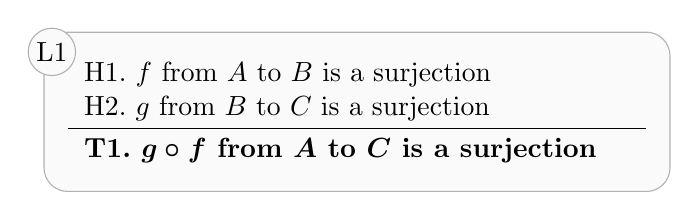
\begin{tikzpicture}[baseline=(main.base)]%
\node[tableau] (main) {%
\\

\begin{tabular}{ll}%
H1.\ $\textrm{$f$ from $A$ to $B$ is a surjection}$&\\
H2.\ $\textrm{$g$ from $B$ to $C$ is a surjection}$&
\Bstrut\\\hline\Tstrut
\textbf{\boldmath T1.\ $\textrm{$g\circ f$ from $A$ to $C$ is a surjection}$\unboldmath }&\textbf{\boldmath \unboldmath }
\end{tabular}%
};%
\node[tableaulabel] at (main.north west) [xshift=4mm, yshift=-5.5mm] {L1};
\end{tikzpicture}%
\end{fit}
\smallskip

\noindent1. Expand pre-universal target T1.\nopagebreak[4] 
\marginpar{}\nopagebreak[4] 
\smallskip\nopagebreak[4] 

\begin{fit}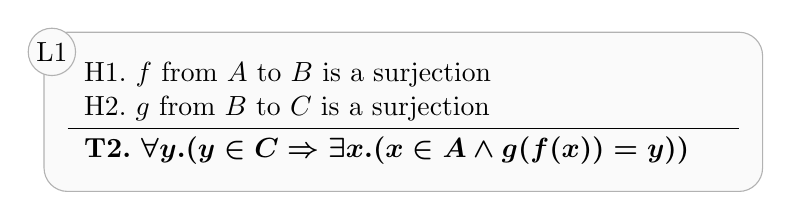
\begin{tikzpicture}[baseline=(main.base)]%
\node[tableau] (main) {%
\\

\begin{tabular}{ll}%
H1.\ $\textrm{$f$ from $A$ to $B$ is a surjection}$&\\
H2.\ $\textrm{$g$ from $B$ to $C$ is a surjection}$&
\Bstrut\\\hline\Tstrut
\textbf{\boldmath T2.\ $\forall y.(\textrm{$y\in C$}\Rightarrow \exists x.(\textrm{$x\in A$}\wedge \textrm{$g(f(x)) = y$}))$\unboldmath }&\textbf{\boldmath \unboldmath }
\end{tabular}%
};%
\node[tableaulabel] at (main.north west) [xshift=4mm, yshift=-5.5mm] {L1};
\end{tikzpicture}%
\end{fit}
\smallskip

\noindent2. Apply `let' trick and move premise of universal-conditional target T2 above the line.\nopagebreak[4] 
\marginpar{Let $y$ be an element of $C$.}\nopagebreak[4] 
\smallskip\nopagebreak[4] 

\begin{fit}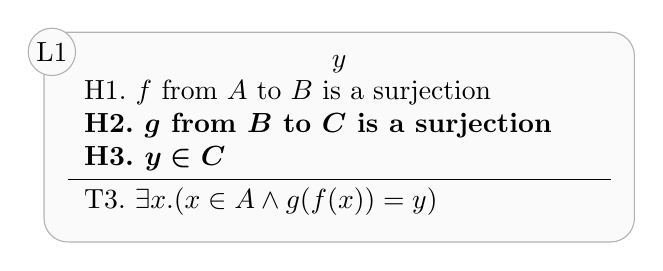
\begin{tikzpicture}[baseline=(main.base)]%
\node[tableau] (main) {%
$y$\\

\begin{tabular}{ll}%
H1.\ $\textrm{$f$ from $A$ to $B$ is a surjection}$&\\
\textbf{\boldmath H2.\ $\textrm{$g$ from $B$ to $C$ is a surjection}$\unboldmath }&\textbf{\boldmath \unboldmath }\\
\textbf{\boldmath H3.\ $\textrm{$y\in C$}$\unboldmath }&\textbf{\boldmath \unboldmath }
\Bstrut\\\hline\Tstrut
T3.\ $\exists x.(\textrm{$x\in A$}\wedge \textrm{$g(f(x)) = y$})$&
\end{tabular}%
};%
\node[tableaulabel] at (main.north west) [xshift=4mm, yshift=-5.5mm] {L1};
\end{tikzpicture}%
\end{fit}
\smallskip

\noindent3. Forwards reasoning using H2 with H3.\nopagebreak[4] 
\marginpar{Since $g$ from $B$ to $C$ is a surjection and $y\in C$, there exists $u\in B$ such that $g(u) = y$.}\nopagebreak[4] 
\smallskip\nopagebreak[4] 

\begin{fit}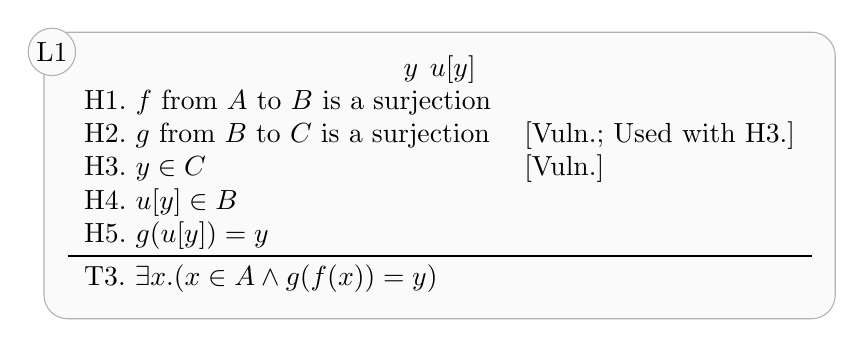
\begin{tikzpicture}[baseline=(main.base)]%
\node[tableau] (main) {%
$y$\hspace{1.5mm}$u[y]$\\

\begin{tabular}{ll}%
H1.\ $\textrm{$f$ from $A$ to $B$ is a surjection}$&\\
H2.\ $\textrm{$g$ from $B$ to $C$ is a surjection}$&[Vuln.; Used with H3.]\\
H3.\ $\textrm{$y\in C$}$&[Vuln.]\\
H4.\ $\textrm{$u[y]\in B$}$&\\
H5.\ $\textrm{$g(u[y]) = y$}$&
\Bstrut\\\hline\Tstrut
T3.\ $\exists x.(\textrm{$x\in A$}\wedge \textrm{$g(f(x)) = y$})$&
\end{tabular}%
};%
\node[tableaulabel] at (main.north west) [xshift=4mm, yshift=-5.5mm] {L1};
\end{tikzpicture}%
\end{fit}
\smallskip

\noindent4. Deleted H3, as this unexpandable atomic statement is unmatchable.\nopagebreak[4] 
\marginpar{}\nopagebreak[4] 
\smallskip\nopagebreak[4] 

\begin{fit}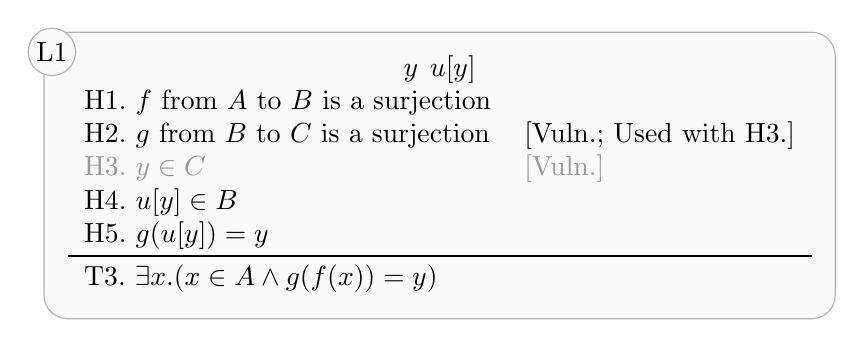
\begin{tikzpicture}[baseline=(main.base)]%
\node[tableau] (main) {%
$y$\hspace{1.5mm}$u[y]$\\

\begin{tabular}{ll}%
H1.\ $\textrm{$f$ from $A$ to $B$ is a surjection}$&\\
H2.\ $\textrm{$g$ from $B$ to $C$ is a surjection}$&[Vuln.; Used with H3.]\\
\grey{H3.\ $\textrm{$y\in C$}$}&\grey{[Vuln.]}\\
H4.\ $\textrm{$u[y]\in B$}$&\\
H5.\ $\textrm{$g(u[y]) = y$}$&
\Bstrut\\\hline\Tstrut
T3.\ $\exists x.(\textrm{$x\in A$}\wedge \textrm{$g(f(x)) = y$})$&
\end{tabular}%
};%
\node[tableaulabel] at (main.north west) [xshift=4mm, yshift=-5.5mm] {L1};
\end{tikzpicture}%
\end{fit}
\smallskip

\noindent5. Delete H2 as no other statement mentions $C$.\nopagebreak[4] 
\marginpar{}\nopagebreak[4] 
\smallskip\nopagebreak[4] 

\begin{fit}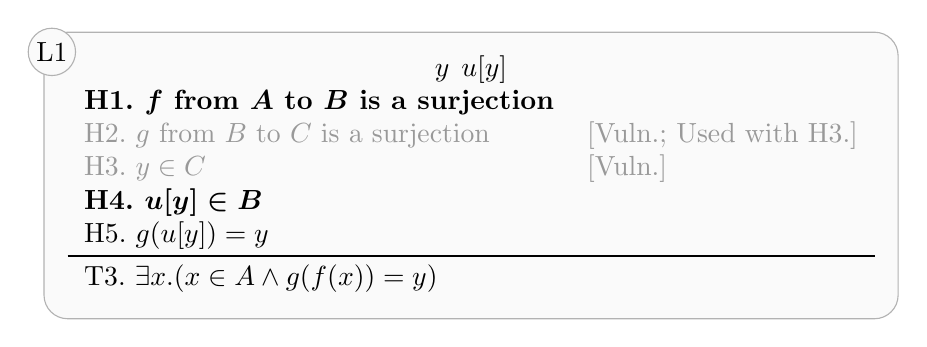
\begin{tikzpicture}[baseline=(main.base)]%
\node[tableau] (main) {%
$y$\hspace{1.5mm}$u[y]$\\

\begin{tabular}{ll}%
\textbf{\boldmath H1.\ $\textrm{$f$ from $A$ to $B$ is a surjection}$\unboldmath }&\textbf{\boldmath \unboldmath }\\
\grey{H2.\ $\textrm{$g$ from $B$ to $C$ is a surjection}$}&\grey{[Vuln.; Used with H3.]}\\
\grey{H3.\ $\textrm{$y\in C$}$}&\grey{[Vuln.]}\\
\textbf{\boldmath H4.\ $\textrm{$u[y]\in B$}$\unboldmath }&\textbf{\boldmath \unboldmath }\\
H5.\ $\textrm{$g(u[y]) = y$}$&
\Bstrut\\\hline\Tstrut
T3.\ $\exists x.(\textrm{$x\in A$}\wedge \textrm{$g(f(x)) = y$})$&
\end{tabular}%
};%
\node[tableaulabel] at (main.north west) [xshift=4mm, yshift=-5.5mm] {L1};
\end{tikzpicture}%
\end{fit}
\smallskip

\noindent6. Forwards reasoning using H1 with H4.\nopagebreak[4] 
\marginpar{Since $f$ from $A$ to $B$ is a surjection and $u\in B$, there exists $v\in A$ such that $f(v) = u$.}\nopagebreak[4] 
\smallskip\nopagebreak[4] 

\begin{fit}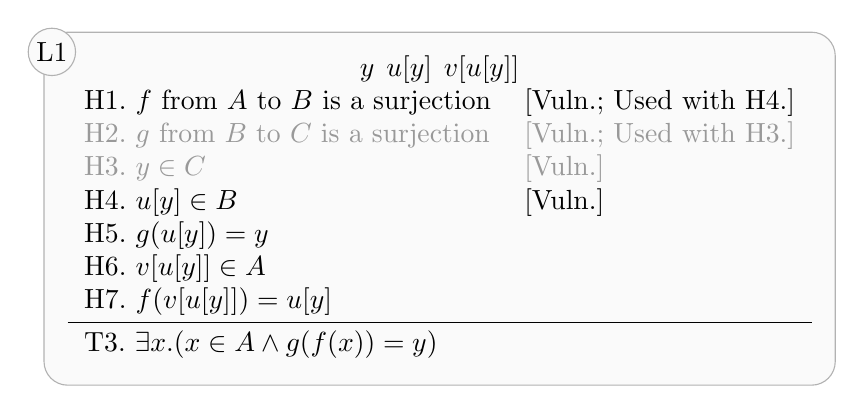
\begin{tikzpicture}[baseline=(main.base)]%
\node[tableau] (main) {%
$y$\hspace{1.5mm}$u[y]$\hspace{1.5mm}$v[u[y]]$\\

\begin{tabular}{ll}%
H1.\ $\textrm{$f$ from $A$ to $B$ is a surjection}$&[Vuln.; Used with H4.]\\
\grey{H2.\ $\textrm{$g$ from $B$ to $C$ is a surjection}$}&\grey{[Vuln.; Used with H3.]}\\
\grey{H3.\ $\textrm{$y\in C$}$}&\grey{[Vuln.]}\\
H4.\ $\textrm{$u[y]\in B$}$&[Vuln.]\\
H5.\ $\textrm{$g(u[y]) = y$}$&\\
H6.\ $\textrm{$v[u[y]]\in A$}$&\\
H7.\ $\textrm{$f(v[u[y]]) = u[y]$}$&
\Bstrut\\\hline\Tstrut
T3.\ $\exists x.(\textrm{$x\in A$}\wedge \textrm{$g(f(x)) = y$})$&
\end{tabular}%
};%
\node[tableaulabel] at (main.north west) [xshift=4mm, yshift=-5.5mm] {L1};
\end{tikzpicture}%
\end{fit}
\smallskip

\noindent7. Deleted H4, as this unexpandable atomic statement is unmatchable.\nopagebreak[4] 
\marginpar{}\nopagebreak[4] 
\smallskip\nopagebreak[4] 

\begin{fit}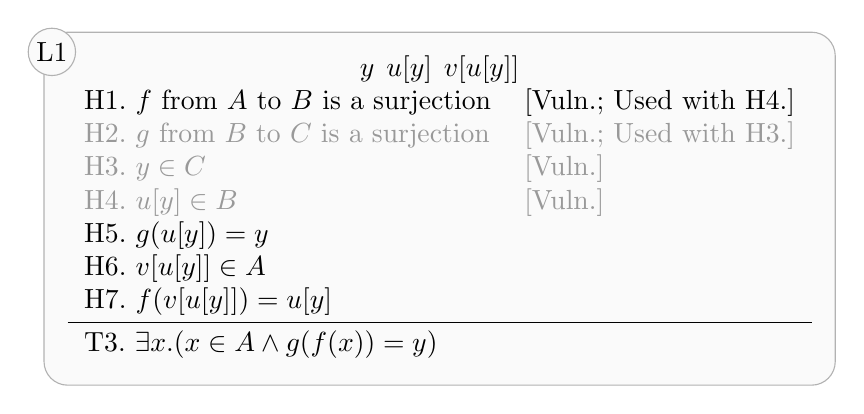
\begin{tikzpicture}[baseline=(main.base)]%
\node[tableau] (main) {%
$y$\hspace{1.5mm}$u[y]$\hspace{1.5mm}$v[u[y]]$\\

\begin{tabular}{ll}%
H1.\ $\textrm{$f$ from $A$ to $B$ is a surjection}$&[Vuln.; Used with H4.]\\
\grey{H2.\ $\textrm{$g$ from $B$ to $C$ is a surjection}$}&\grey{[Vuln.; Used with H3.]}\\
\grey{H3.\ $\textrm{$y\in C$}$}&\grey{[Vuln.]}\\
\grey{H4.\ $\textrm{$u[y]\in B$}$}&\grey{[Vuln.]}\\
H5.\ $\textrm{$g(u[y]) = y$}$&\\
H6.\ $\textrm{$v[u[y]]\in A$}$&\\
H7.\ $\textrm{$f(v[u[y]]) = u[y]$}$&
\Bstrut\\\hline\Tstrut
T3.\ $\exists x.(\textrm{$x\in A$}\wedge \textrm{$g(f(x)) = y$})$&
\end{tabular}%
};%
\node[tableaulabel] at (main.north west) [xshift=4mm, yshift=-5.5mm] {L1};
\end{tikzpicture}%
\end{fit}
\smallskip

\noindent8. Delete H1 as no other statement mentions $B$.\nopagebreak[4] 
\marginpar{}\nopagebreak[4] 
\smallskip\nopagebreak[4] 

\begin{fit}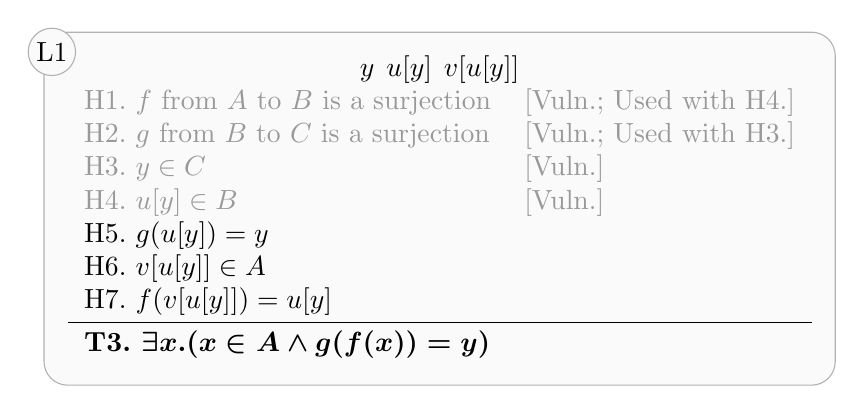
\begin{tikzpicture}[baseline=(main.base)]%
\node[tableau] (main) {%
$y$\hspace{1.5mm}$u[y]$\hspace{1.5mm}$v[u[y]]$\\

\begin{tabular}{ll}%
\grey{H1.\ $\textrm{$f$ from $A$ to $B$ is a surjection}$}&\grey{[Vuln.; Used with H4.]}\\
\grey{H2.\ $\textrm{$g$ from $B$ to $C$ is a surjection}$}&\grey{[Vuln.; Used with H3.]}\\
\grey{H3.\ $\textrm{$y\in C$}$}&\grey{[Vuln.]}\\
\grey{H4.\ $\textrm{$u[y]\in B$}$}&\grey{[Vuln.]}\\
H5.\ $\textrm{$g(u[y]) = y$}$&\\
H6.\ $\textrm{$v[u[y]]\in A$}$&\\
H7.\ $\textrm{$f(v[u[y]]) = u[y]$}$&
\Bstrut\\\hline\Tstrut
\textbf{\boldmath T3.\ $\exists x.(\textrm{$x\in A$}\wedge \textrm{$g(f(x)) = y$})$\unboldmath }&\textbf{\boldmath \unboldmath }
\end{tabular}%
};%
\node[tableaulabel] at (main.north west) [xshift=4mm, yshift=-5.5mm] {L1};
\end{tikzpicture}%
\end{fit}
\smallskip

\noindent9. Unlock existential target T3.\nopagebreak[4] 
\marginpar{We would like to find $x\in A$ s.t. $g(f(x)) = y$.}\nopagebreak[4] 
\smallskip\nopagebreak[4] 

\begin{fit}\begin{tikzpicture}[baseline=(main.base)]%
\node[tableau] (main) {%
$y$\hspace{1.5mm}$u[y]$\hspace{1.5mm}$v[u[y]]$\\

\begin{tabular}{ll}%
\grey{H1.\ $\textrm{$f$ from $A$ to $B$ is a surjection}$}&\grey{[Vuln.; Used with H4.]}\\
\grey{H2.\ $\textrm{$g$ from $B$ to $C$ is a surjection}$}&\grey{[Vuln.; Used with H3.]}\\
\grey{H3.\ $\textrm{$y\in C$}$}&\grey{[Vuln.]}\\
\grey{H4.\ $\textrm{$u[y]\in B$}$}&\grey{[Vuln.]}\\
H5.\ $\textrm{$g(u[y]) = y$}$&\\
H6.\ $\textrm{$v[u[y]]\in A$}$&\\
H7.\ $\textrm{$f(v[u[y]]) = u[y]$}$&
\Bstrut\\\hline\Tstrut
\begin{tikzpicture}[baseline=(main.base)]%
\node[tableau] (main) {%
$x^\blacklozenge $\\

\begin{tabular}{ll}%

\Bstrut\\\hline\Tstrut
T4.\ $\textrm{$x^\blacklozenge \in A$}$&\\
T5.\ $\textrm{$g(f(x^\blacklozenge )) = y$}$&
\end{tabular}%
};%
\node[tableaulabel] at (main.north west) [xshift=4mm, yshift=-5.5mm] {L2$^\blacklozenge$};
\end{tikzpicture}%

\end{tabular}%
};%
\node[tableaulabel] at (main.north west) [xshift=4mm, yshift=-5.5mm] {L1};
\end{tikzpicture}%
\end{fit}

No moves possible.
\cleardoublepage

\end{steps}
{\begin{center} \large \textbf{If $f$ is an injection then $f(A)\cap f(B)\subset f(A\cap B)$}\end{center}}\nopagebreak[4]

\begin{center}
\begin{minipage}{120mm}
Let $x$ be an element of $f(A)\cap f(B)$. Then $x\in f(A)$ and $x\in f(B)$. That is, there exists $y\in A$ such that $f(y) = x$ and there exists $z\in B$ such that $f(z) = x$. Since $f$ is an injection, $f(y) = x$ and $f(z) = x$, we have that $y = z$. We would like to find $u\in A\cap B$ s.t. $f(u) = x$. But $u\in A\cap B$ if and only if $u\in A$ and $u\in B$. Since $y = z$, we have that $y\in B$. Therefore, setting $u = y$, we are done.
\end{minipage}
\end{center}

\bigskip
\begin{steps}
\begin{fit}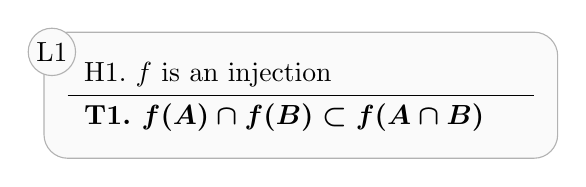
\begin{tikzpicture}[baseline=(main.base)]%
\node[tableau] (main) {%
\\

\begin{tabular}{ll}%
H1.\ $\textrm{$f$ is an injection}$&
\Bstrut\\\hline\Tstrut
\textbf{\boldmath T1.\ $\textrm{$f(A)\cap f(B)\subset f(A\cap B)$}$\unboldmath }&\textbf{\boldmath \unboldmath }
\end{tabular}%
};%
\node[tableaulabel] at (main.north west) [xshift=4mm, yshift=-5.5mm] {L1};
\end{tikzpicture}%
\end{fit}
\smallskip

\noindent1. Expand pre-universal target T1.\nopagebreak[4] 
\marginpar{}\nopagebreak[4] 
\smallskip\nopagebreak[4] 

\begin{fit}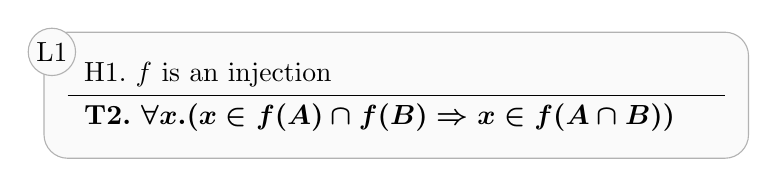
\begin{tikzpicture}[baseline=(main.base)]%
\node[tableau] (main) {%
\\

\begin{tabular}{ll}%
H1.\ $\textrm{$f$ is an injection}$&
\Bstrut\\\hline\Tstrut
\textbf{\boldmath T2.\ $\forall x.(\textrm{$x\in f(A)\cap f(B)$}\Rightarrow \textrm{$x\in f(A\cap B)$})$\unboldmath }&\textbf{\boldmath \unboldmath }
\end{tabular}%
};%
\node[tableaulabel] at (main.north west) [xshift=4mm, yshift=-5.5mm] {L1};
\end{tikzpicture}%
\end{fit}
\smallskip

\noindent2. Apply `let' trick and move premise of universal-conditional target T2 above the line.\nopagebreak[4] 
\marginpar{Let $x$ be an element of $f(A)\cap f(B)$.}\nopagebreak[4] 
\smallskip\nopagebreak[4] 

\begin{fit}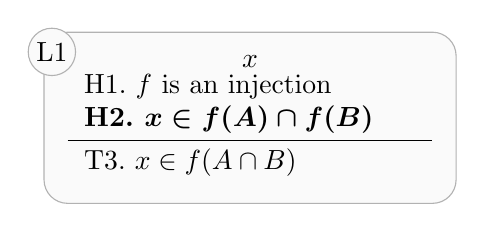
\begin{tikzpicture}[baseline=(main.base)]%
\node[tableau] (main) {%
$x$\\

\begin{tabular}{ll}%
H1.\ $\textrm{$f$ is an injection}$&\\
\textbf{\boldmath H2.\ $\textrm{$x\in f(A)\cap f(B)$}$\unboldmath }&\textbf{\boldmath \unboldmath }
\Bstrut\\\hline\Tstrut
T3.\ $\textrm{$x\in f(A\cap B)$}$&
\end{tabular}%
};%
\node[tableaulabel] at (main.north west) [xshift=4mm, yshift=-5.5mm] {L1};
\end{tikzpicture}%
\end{fit}
\smallskip

\noindent3. Quantifier-free expansion of hypothesis H2.\nopagebreak[4] 
\marginpar{Since $x\in f(A)\cap f(B)$, $x\in f(A)$ and $x\in f(B)$.}\nopagebreak[4] 
\smallskip\nopagebreak[4] 

\begin{fit}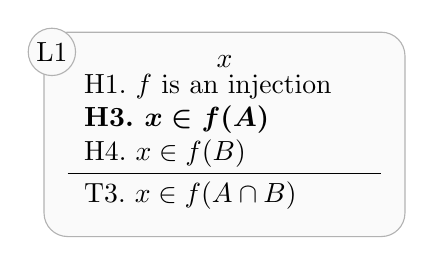
\begin{tikzpicture}[baseline=(main.base)]%
\node[tableau] (main) {%
$x$\\

\begin{tabular}{ll}%
H1.\ $\textrm{$f$ is an injection}$&\\
\textbf{\boldmath H3.\ $\textrm{$x\in f(A)$}$\unboldmath }&\textbf{\boldmath \unboldmath }\\
H4.\ $\textrm{$x\in f(B)$}$&
\Bstrut\\\hline\Tstrut
T3.\ $\textrm{$x\in f(A\cap B)$}$&
\end{tabular}%
};%
\node[tableaulabel] at (main.north west) [xshift=4mm, yshift=-5.5mm] {L1};
\end{tikzpicture}%
\end{fit}
\smallskip

\noindent4. Expand pre-existential hypothesis H3.\nopagebreak[4] 
\marginpar{By definition, since $x\in f(A)$, there exists $y\in A$ such that $f(y) = x$.}\nopagebreak[4] 
\smallskip\nopagebreak[4] 

\begin{fit}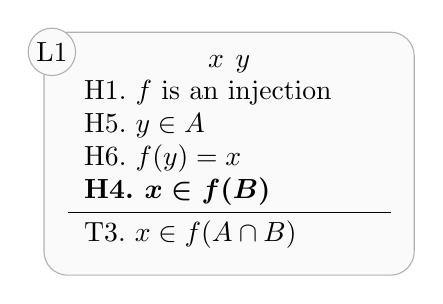
\begin{tikzpicture}[baseline=(main.base)]%
\node[tableau] (main) {%
$x$\hspace{1.5mm}$y$\\

\begin{tabular}{ll}%
H1.\ $\textrm{$f$ is an injection}$&\\
H5.\ $\textrm{$y\in A$}$&\\
H6.\ $\textrm{$f(y) = x$}$&\\
\textbf{\boldmath H4.\ $\textrm{$x\in f(B)$}$\unboldmath }&\textbf{\boldmath \unboldmath }
\Bstrut\\\hline\Tstrut
T3.\ $\textrm{$x\in f(A\cap B)$}$&
\end{tabular}%
};%
\node[tableaulabel] at (main.north west) [xshift=4mm, yshift=-5.5mm] {L1};
\end{tikzpicture}%
\end{fit}
\smallskip

\noindent5. Expand pre-existential hypothesis H4.\nopagebreak[4] 
\marginpar{By definition, since $x\in f(B)$, there exists $z\in B$ such that $f(z) = x$.}\nopagebreak[4] 
\smallskip\nopagebreak[4] 

\begin{fit}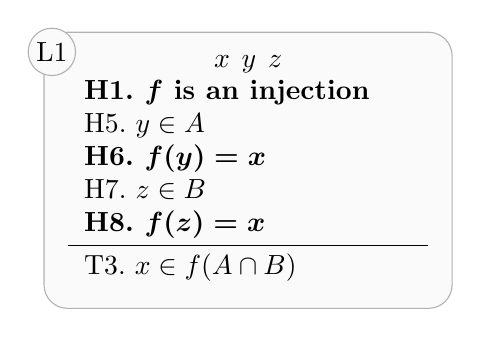
\begin{tikzpicture}[baseline=(main.base)]%
\node[tableau] (main) {%
$x$\hspace{1.5mm}$y$\hspace{1.5mm}$z$\\

\begin{tabular}{ll}%
\textbf{\boldmath H1.\ $\textrm{$f$ is an injection}$\unboldmath }&\textbf{\boldmath \unboldmath }\\
H5.\ $\textrm{$y\in A$}$&\\
\textbf{\boldmath H6.\ $\textrm{$f(y) = x$}$\unboldmath }&\textbf{\boldmath \unboldmath }\\
H7.\ $\textrm{$z\in B$}$&\\
\textbf{\boldmath H8.\ $\textrm{$f(z) = x$}$\unboldmath }&\textbf{\boldmath \unboldmath }
\Bstrut\\\hline\Tstrut
T3.\ $\textrm{$x\in f(A\cap B)$}$&
\end{tabular}%
};%
\node[tableaulabel] at (main.north west) [xshift=4mm, yshift=-5.5mm] {L1};
\end{tikzpicture}%
\end{fit}
\smallskip

\noindent6. Forwards reasoning using H1 with (H6,H8).\nopagebreak[4] 
\marginpar{Since $f$ is an injection, $f(y) = x$ and $f(z) = x$, we have that $y = z$.}\nopagebreak[4] 
\smallskip\nopagebreak[4] 

\begin{fit}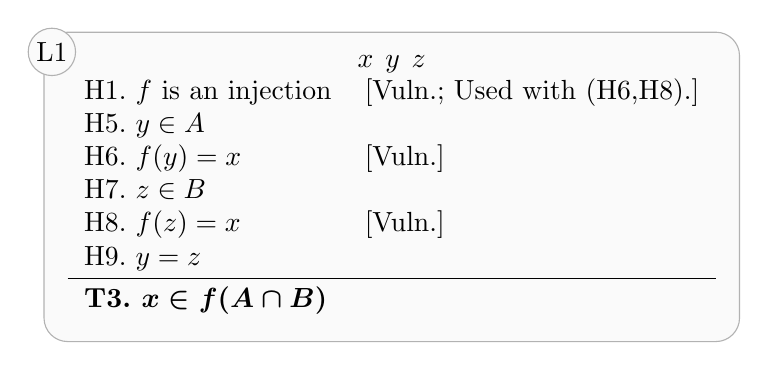
\begin{tikzpicture}[baseline=(main.base)]%
\node[tableau] (main) {%
$x$\hspace{1.5mm}$y$\hspace{1.5mm}$z$\\

\begin{tabular}{ll}%
H1.\ $\textrm{$f$ is an injection}$&[Vuln.; Used with (H6,H8).]\\
H5.\ $\textrm{$y\in A$}$&\\
H6.\ $\textrm{$f(y) = x$}$&[Vuln.]\\
H7.\ $\textrm{$z\in B$}$&\\
H8.\ $\textrm{$f(z) = x$}$&[Vuln.]\\
H9.\ $\textrm{$y = z$}$&
\Bstrut\\\hline\Tstrut
\textbf{\boldmath T3.\ $\textrm{$x\in f(A\cap B)$}$\unboldmath }&\textbf{\boldmath \unboldmath }
\end{tabular}%
};%
\node[tableaulabel] at (main.north west) [xshift=4mm, yshift=-5.5mm] {L1};
\end{tikzpicture}%
\end{fit}
\smallskip

\noindent7. Expand pre-existential target T3.\nopagebreak[4] 
\marginpar{We would like to find $u\in A\cap B$ s.t. $f(u) = x$.}\nopagebreak[4] 
\smallskip\nopagebreak[4] 

\begin{fit}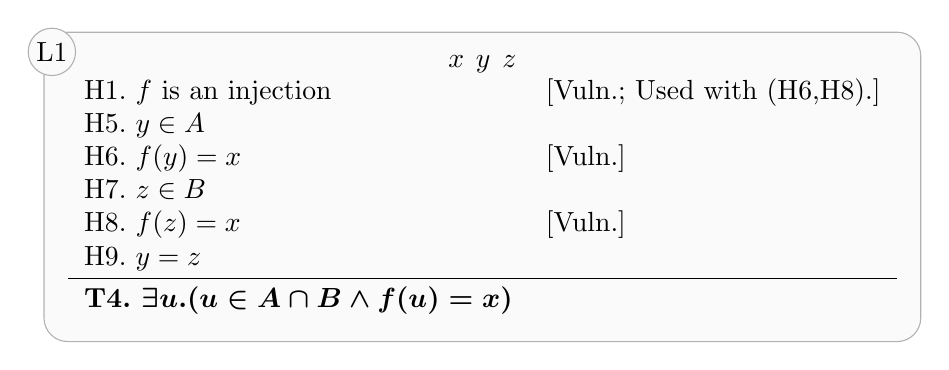
\begin{tikzpicture}[baseline=(main.base)]%
\node[tableau] (main) {%
$x$\hspace{1.5mm}$y$\hspace{1.5mm}$z$\\

\begin{tabular}{ll}%
H1.\ $\textrm{$f$ is an injection}$&[Vuln.; Used with (H6,H8).]\\
H5.\ $\textrm{$y\in A$}$&\\
H6.\ $\textrm{$f(y) = x$}$&[Vuln.]\\
H7.\ $\textrm{$z\in B$}$&\\
H8.\ $\textrm{$f(z) = x$}$&[Vuln.]\\
H9.\ $\textrm{$y = z$}$&
\Bstrut\\\hline\Tstrut
\textbf{\boldmath T4.\ $\exists u.(\textrm{$u\in A\cap B$}\wedge \textrm{$f(u) = x$})$\unboldmath }&\textbf{\boldmath \unboldmath }
\end{tabular}%
};%
\node[tableaulabel] at (main.north west) [xshift=4mm, yshift=-5.5mm] {L1};
\end{tikzpicture}%
\end{fit}
\smallskip

\noindent8. Unlock existential target T4.\nopagebreak[4] 
\marginpar{We would like to find $u\in A\cap B$ s.t. $f(u) = x$.}\nopagebreak[4] 
\smallskip\nopagebreak[4] 

\begin{fit}\begin{tikzpicture}[baseline=(main.base)]%
\node[tableau] (main) {%
$x$\hspace{1.5mm}$y$\hspace{1.5mm}$z$\\

\begin{tabular}{ll}%
H1.\ $\textrm{$f$ is an injection}$&[Vuln.; Used with (H6,H8).]\\
H5.\ $\textrm{$y\in A$}$&\\
H6.\ $\textrm{$f(y) = x$}$&[Vuln.]\\
H7.\ $\textrm{$z\in B$}$&\\
H8.\ $\textrm{$f(z) = x$}$&[Vuln.]\\
H9.\ $\textrm{$y = z$}$&
\Bstrut\\\hline\Tstrut
\begin{tikzpicture}[baseline=(main.base)]%
\node[tableau] (main) {%
$u^\blacklozenge $\\

\begin{tabular}{ll}%

\Bstrut\\\hline\Tstrut
\textbf{\boldmath T5.\ $\textrm{$u^\blacklozenge \in A\cap B$}$\unboldmath }&\textbf{\boldmath \unboldmath }\\
T6.\ $\textrm{$f(u^\blacklozenge ) = x$}$&
\end{tabular}%
};%
\node[tableaulabel] at (main.north west) [xshift=4mm, yshift=-5.5mm] {L2$^\blacklozenge$};
\end{tikzpicture}%

\end{tabular}%
};%
\node[tableaulabel] at (main.north west) [xshift=4mm, yshift=-5.5mm] {L1};
\end{tikzpicture}%
\end{fit}
\smallskip

\noindent9. Quantifier-free expansion of target T5.\nopagebreak[4] 
\marginpar{But $u\in A\cap B$ if and only if $u\in A$ and $u\in B$.}\nopagebreak[4] 
\smallskip\nopagebreak[4] 

\begin{fit}\begin{tikzpicture}[baseline=(main.base)]%
\node[tableau] (main) {%
$x$\hspace{1.5mm}$y$\hspace{1.5mm}$z$\\

\begin{tabular}{ll}%
H1.\ $\textrm{$f$ is an injection}$&[Vuln.; Used with (H6,H8).]\\
H5.\ $\textrm{$y\in A$}$&\\
H6.\ $\textrm{$f(y) = x$}$&[Vuln.]\\
H7.\ $\textrm{$z\in B$}$&\\
H8.\ $\textrm{$f(z) = x$}$&[Vuln.]\\
\textbf{\boldmath H9.\ $\textrm{$y = z$}$\unboldmath }&\textbf{\boldmath \unboldmath }
\Bstrut\\\hline\Tstrut
\begin{tikzpicture}[baseline=(main.base)]%
\node[tableau] (main) {%
$u^\blacklozenge $\\

\begin{tabular}{ll}%

\Bstrut\\\hline\Tstrut
T7.\ $\textrm{$u^\blacklozenge \in A$}$&\\
T8.\ $\textrm{$u^\blacklozenge \in B$}$&\\
T6.\ $\textrm{$f(u^\blacklozenge ) = x$}$&
\end{tabular}%
};%
\node[tableaulabel] at (main.north west) [xshift=4mm, yshift=-5.5mm] {L2$^\blacklozenge$};
\end{tikzpicture}%

\end{tabular}%
};%
\node[tableaulabel] at (main.north west) [xshift=4mm, yshift=-5.5mm] {L1};
\end{tikzpicture}%
\end{fit}
\smallskip

\noindent10. Rewrite $z$ as $y$ throughout the tableau using hypothesis H9.\nopagebreak[4] 
\marginpar{Since $y = z$, we have that $y\in B$.}\nopagebreak[4] 
\smallskip\nopagebreak[4] 

\begin{fit}\begin{tikzpicture}[baseline=(main.base)]%
\node[tableau] (main) {%
$x$\hspace{1.5mm}$y$\hspace{1.5mm}$z$\\

\begin{tabular}{ll}%
H1.\ $\textrm{$f$ is an injection}$&[Vuln.; Used with (H6,H8).]\\
H5.\ $\textrm{$y\in A$}$&\\
H6.\ $\textrm{$f(y) = x$}$&[Vuln.]\\
H10.\ $\textrm{$y\in B$}$&
\Bstrut\\\hline\Tstrut
\begin{tikzpicture}[baseline=(main.base)]%
\node[tableau] (main) {%
$u^\blacklozenge $\\

\begin{tabular}{ll}%

\Bstrut\\\hline\Tstrut
T7.\ $\textrm{$u^\blacklozenge \in A$}$&\\
T8.\ $\textrm{$u^\blacklozenge \in B$}$&\\
T6.\ $\textrm{$f(u^\blacklozenge ) = x$}$&
\end{tabular}%
};%
\node[tableaulabel] at (main.north west) [xshift=4mm, yshift=-5.5mm] {L2$^\blacklozenge$};
\end{tikzpicture}%

\end{tabular}%
};%
\node[tableaulabel] at (main.north west) [xshift=4mm, yshift=-5.5mm] {L1};
\end{tikzpicture}%
\end{fit}
\smallskip

\noindent11. Moved H6 down, as $x$ can only be utilised by T6.\nopagebreak[4] 
\marginpar{}\nopagebreak[4] 
\smallskip\nopagebreak[4] 

\begin{fit}\begin{tikzpicture}[baseline=(main.base)]%
\node[tableau] (main) {%
$x$\hspace{1.5mm}$y$\hspace{1.5mm}$z$\\

\begin{tabular}{ll}%
H1.\ $\textrm{$f$ is an injection}$&[Vuln.; Used with (H6,H8).]\\
H5.\ $\textrm{$y\in A$}$&\\
H10.\ $\textrm{$y\in B$}$&
\Bstrut\\\hline\Tstrut
\begin{tikzpicture}[baseline=(main.base)]%
\node[tableau] (main) {%
$u^\blacklozenge $\\

\begin{tabular}{ll}%

\Bstrut\\\hline\Tstrut
T7.\ $\textrm{$u^\blacklozenge \in A$}$&\\
T8.\ $\textrm{$u^\blacklozenge \in B$}$&\\
\begin{tikzpicture}[baseline=(main.base)]%
\node[tableau] (main) {%
\\

\begin{tabular}{ll}%
H6.\ $\textrm{$f(y) = x$}$&[Vuln.; From L1.]
\Bstrut\\\hline\Tstrut
T6.\ $\textrm{$f(u^\blacklozenge ) = x$}$&
\end{tabular}%
};%
\node[tableaulabel] at (main.north west) [xshift=4mm, yshift=-5.5mm] {L3};
\end{tikzpicture}%

\end{tabular}%
};%
\node[tableaulabel] at (main.north west) [xshift=4mm, yshift=-5.5mm] {L2$^\blacklozenge$};
\end{tikzpicture}%

\end{tabular}%
};%
\node[tableaulabel] at (main.north west) [xshift=4mm, yshift=-5.5mm] {L1};
\end{tikzpicture}%
\end{fit}
\smallskip

\noindent12. Choosing $u^\blacklozenge  = y$ matches all targets inside L2$^\blacklozenge$ against hypotheses, so L2$^\blacklozenge$ is done.\nopagebreak[4] 
\marginpar{Therefore, setting $u = y$, we are done.}\nopagebreak[4] 
\smallskip\nopagebreak[4] 

\begin{fit}\begin{tikzpicture}[baseline=(main.base)]%
\node[tableau] (main) {%
$x$\hspace{1.5mm}$y$\hspace{1.5mm}$z$\\

\begin{tabular}{ll}%
H1.\ $\textrm{$f$ is an injection}$&[Vuln.; Used with (H6,H8).]\\
H5.\ $\textrm{$y\in A$}$&\\
H10.\ $\textrm{$y\in B$}$&
\Bstrut\\\hline\Tstrut
\begin{tikzpicture}%
\node[tableau] (main) {%
\ \ \,Done
};%
\node[tableaulabel] at (main.north west) [xshift=4mm, yshift=-5.5mm] {L2$^\blacklozenge$};
\end{tikzpicture}%

\end{tabular}%
};%
\node[tableaulabel] at (main.north west) [xshift=4mm, yshift=-5.5mm] {L1};
\end{tikzpicture}%
\end{fit}
\smallskip

\noindent13. All targets of L1 are `Done', so L1 is itself done.\nopagebreak[4] 
\marginpar{}\nopagebreak[4] 
\smallskip\nopagebreak[4] 

\begin{fit}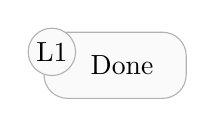
\begin{tikzpicture}%
\node[tableau] (main) {%
\ \ \,Done
};%
\node[tableaulabel] at (main.north west) [xshift=4mm, yshift=-5.5mm] {L1};
\end{tikzpicture}%
\end{fit}

Problem solved.
\cleardoublepage

\end{steps}

\end{document}
